\subsection{Tenant names}
\label{sec:application:building_the_model:tenant_names}

In the ninth step, the tenants are named. Formally, the $\type{name}$ attribute on the $.\type{Tenant}$ class is introduced, including its values. As before, \cref{subsec:library_of_transformations:type_level_transformations:data_fields} is used to introduce the field, while on the instance level, \cref{subsec:library_of_transformations:instance_level_transformations:data_field_values} is used to introduce the values.

The $classtype$ of the new field is $.\type{Tenant}$, as the field will be defined for tenants. The $name$ of the new field is $\type{name}$ and the $fieldtype$ is $\type{string}$. The set of objects of which the value is set is is equal to all tenant objects, so $objects = \{Tenant1, Tenant2, Tenant3, Tenant4, Tenant5\}$. The function for $obids$ returns the existing identifier of each of these objects. The $values$ function is defined as follows:
\begin{align*}
    values = values = \{&(Tenant1, \text{``B.R. Mankjon''}), (Tenant2, \text{``P.J.R. Nam''}), (Tenant3, \text{``L. Horn''}), \\&(Tenant4, \text{``A.C.C. Turg''}), (Tenant5, \text{``M. Silon''})\}
\end{align*}

The following model is obtained:

\LTXtable{\textwidth}{tex/06_application/02_building_the_model/tables/09_tenant_names.tex}

\begin{figure}[p]
    \centering
    \begin{subfigure}{0.98\textwidth}
        \centering
        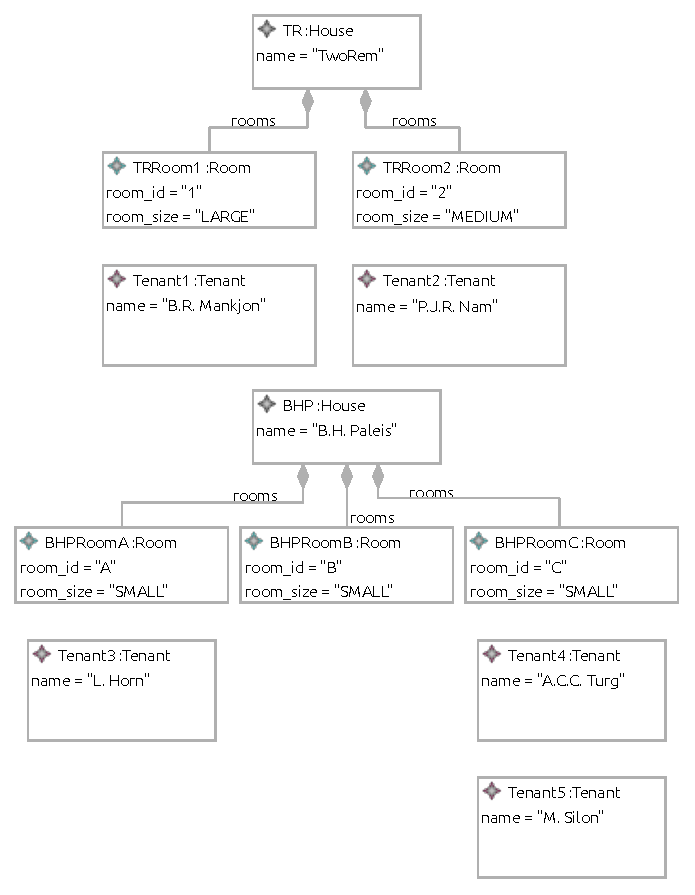
\includegraphics{images/06_application/instance_model/step09.pdf}
        \caption{Instance Model $Im_9$}
        \label{fig:application:building_the_model:tenant_names:ecore:instance_model}
    \end{subfigure}
    \\
    \begin{subfigure}{0.98\textwidth}
        \centering
        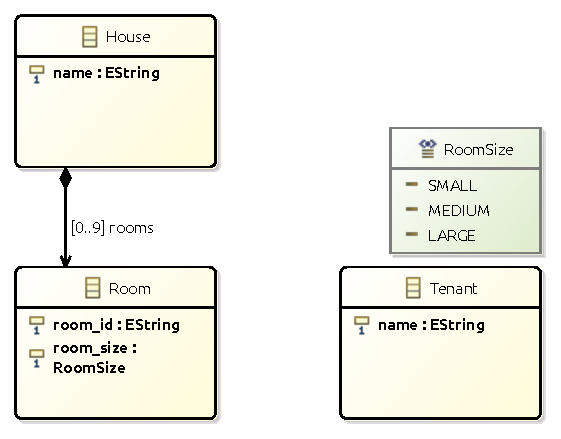
\includegraphics{images/06_application/type_model/step09.pdf}
        \caption{Type Model $Tm_9$}
        \label{fig:application:building_the_model:tenant_names:ecore:type_model}
    \end{subfigure}
    \caption{The Ecore model after step 9}
    \label{fig:application:building_the_model:tenant_names:ecore}
\end{figure}

\begin{figure}[p]
    \centering
    \begin{subfigure}{0.98\textwidth}
        \centering
        % To use this figure in your LaTeX document
% import the package groove/resources/groove2tikz.sty
%
\begin{tikzpicture}[scale=\tikzscale,name prefix=step09-]
\node[type_node] (n0) at (0.740, -0.400) {\ml{\textbf{House}\\name: \textbf{string}}};
\node[type_node] (n1) at (0.730, -1.585) {\ml{\textbf{Room}\\room\_id: \textbf{string}}};
\node[type_node] (n2) at (2.380, -0.560) {\ml{\textbf{RoomSize}\\\textit{LARGE}\\\textit{MEDIUM}\\\textit{SMALL}}};
\node[type_node] (n3) at (2.500, -1.590) {\ml{\textbf{Tenant}\\name: \textbf{string}}};

\path[basic_edge, composite](n0.south -| 0.730, -1.585) -- node[lab] {\ml{rooms}} (n1) ;
\path[basic_edge] (n1)  -- node[lab] {\ml{room\_size}} (n2) ;
\end{tikzpicture}

        \caption{Instance Graph $IG_9$}
        \label{fig:application:building_the_model:tenant_names:groove:instance_graph}
    \end{subfigure}
    \\
    \begin{subfigure}{0.98\textwidth}
        \centering
        % To use this figure in your LaTeX document
% import the package groove/resources/groove2tikz.sty
%
\begin{tikzpicture}[scale=\tikzscale,name prefix=step09-]
\node[type_node] (n0) at (0.740, -0.400) {\ml{\textbf{House}\\name: \textbf{string}}};
\node[type_node] (n1) at (0.730, -1.585) {\ml{\textbf{Room}\\room\_id: \textbf{string}}};
\node[type_node] (n2) at (2.380, -0.560) {\ml{\textbf{RoomSize}\\\textit{LARGE}\\\textit{MEDIUM}\\\textit{SMALL}}};
\node[type_node] (n3) at (2.500, -1.590) {\ml{\textbf{Tenant}\\name: \textbf{string}}};

\path[basic_edge, composite](n0.south -| 0.730, -1.585) -- node[lab] {\ml{rooms}} (n1) ;
\path[basic_edge] (n1)  -- node[lab] {\ml{room\_size}} (n2) ;
\end{tikzpicture}

        \caption{Type Graph $TG_9$}
        \label{fig:application:building_the_model:tenant_names:groove:type_graph}
    \end{subfigure}
    \caption{The GROOVE graphs after step 9}
    \label{fig:application:building_the_model:tenant_names:groove}
\end{figure}

A visual representation of $Tm_9$ and $Im_9$ can be found in \cref{fig:application:building_the_model:tenant_names:ecore}. Similarly, a visual representation of $TG_9$ and $IG_9$ can be found in \cref{fig:application:building_the_model:tenant_names:groove}. Please note that because of the definitions of $f_9(Im_9)$ and $f'_9(IG_9)$, we have that $f_9(Im_9) = IG_9$ and $f'_9(IG_9) = Im_9$. Furthermore, $f_9(Im_9)$ and $f'_9(IG_9)$ are valid mapping functions themselves, such that they can be combined with another mapping function in the next step.

Just like the other types, it is possible to introduce fields for the tenant objects. This way, even types that are introduced later on can be enriched with new information. The visualisation shows the different names set for the tenants in both the Ecore model and GROOVE graphs.

\afterpage{\FloatBarrier}